\begin{appendix}
    \section{数据\label{appendix:数据}}
    以下为官方发布的疫情数据:
    \\
    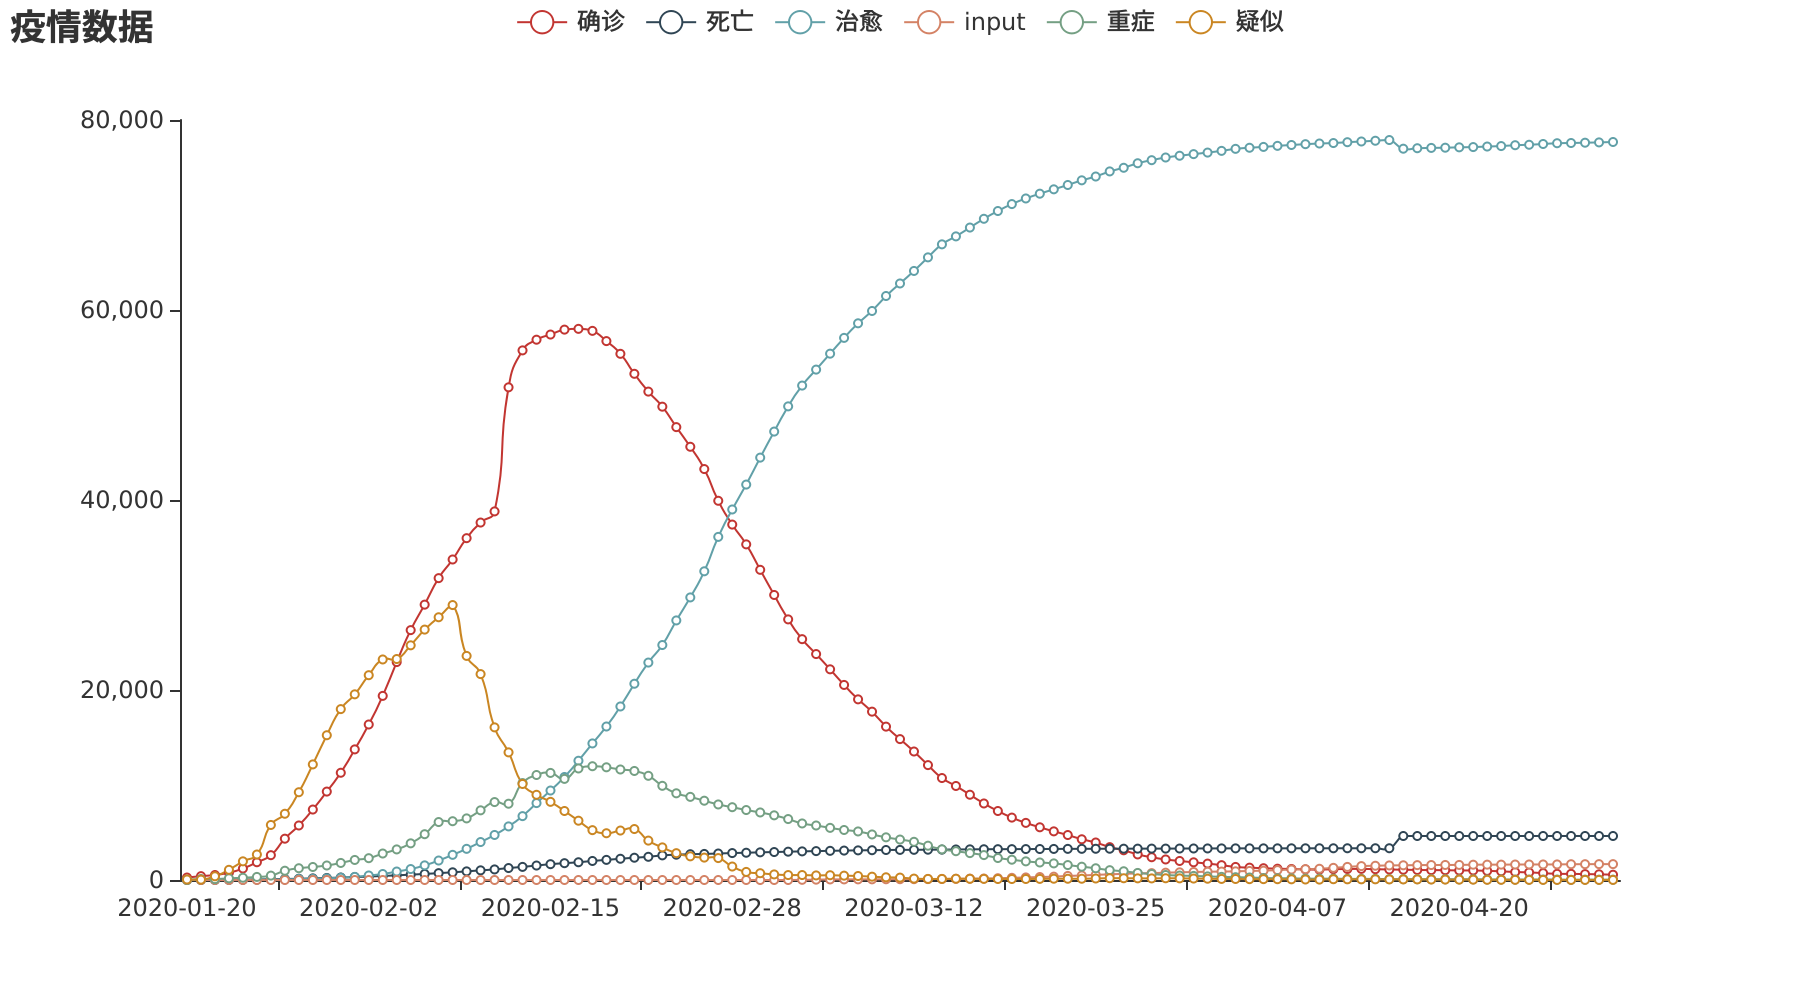
\includegraphics[width=\imagewidth]{疫情数据.png}
    \\
    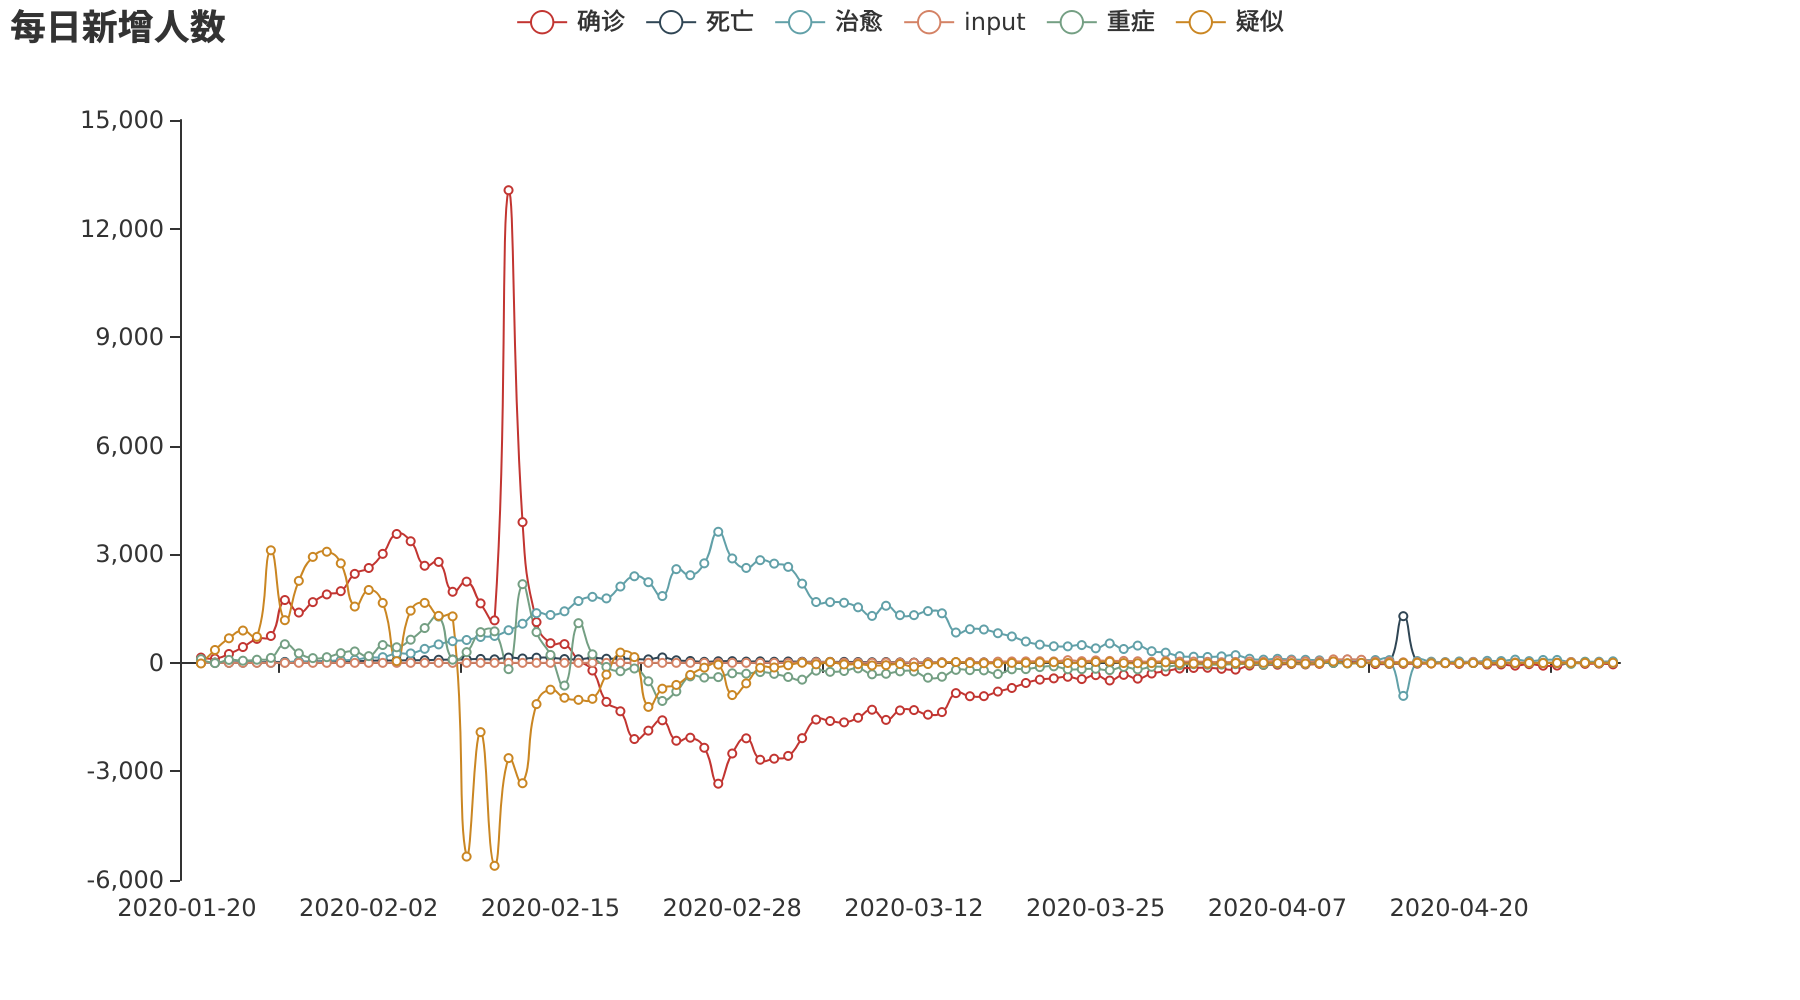
\includegraphics[width=\imagewidth]{每日新增人数.png}
    \par
    2月12日确诊人数猛增,
    是因为当日重新规定了确诊条件,
    导致许多疑似病例纳入确诊人数。
    \section{模型积分式\label{appendix:模型积分式}}
    \begin{table}[H]
        \centering
        \caption{人群}
        \begin{tabular}{ll}
            \hline
            符号 & 含义   \\
            \hline
            $S$  & 易感者 \\
            $I$  & 感染者 \\
            $R$  & 康复者 \\
            $E$  & 携带者 \\
            $D$  & 病逝者 \\
            \hline
        \end{tabular}
    \end{table}
    \subsection{SIR}
    \begin{table}[H]
        \centering
        \caption{SIR模型参数表}
        \begin{tabular}{ll}
            \hline
            符号     & 含义         \\
            \hline
            $\alpha$ & \PText{S}{I} \\
            $\beta$  & \PText{I}{R} \\
            \hline
        \end{tabular}
    \end{table}
    \def\SI{IS\alpha}
    \def\IR{I\beta}
    \begin{align}
        \dt{S} & = -\SI      \\
        \dt{I} & = \SI - \IR \\
        \dt{R} & = \IR
    \end{align}
    \subsection{SEIR}
    \begin{table}[H]
        \centering
        \caption{SEIR模型参数表}
        \begin{tabular}{ll}
            \hline
            符号     & 含义         \\
            \hline
            $\alpha$ & \PText{S}{E} \\
            $\gamma$ & \PText{E}{I} \\
            $\beta$  & \PText{I}{R} \\
            \hline
        \end{tabular}
    \end{table}
    \def\SE{(I+E)S\alpha}
    \def\EI{E\gamma}
    \def\IR{I\beta}
    \begin{align}
        \dt{S} & = -\SE      \\
        \dt{E} & = \SE - \EI \\
        \dt{I} & = \EI - \IR \\
        \dt{R} & = \IR
    \end{align}
    \subsection{SEIRD}
    \begin{table}[H]
        \centering
        \caption{SEIRD模型参数表}
        \begin{tabular}{ll}
            \hline
            符号     & 含义         \\
            \hline
            $\alpha$ & \PText{S}{E} \\
            $\gamma$ & \PText{E}{I} \\
            $\beta$  & \PText{I}{R} \\
            $\delta$ & \PText{I}{D} \\
            \hline
        \end{tabular}
    \end{table}
    \def\SE{(I+E)S\alpha}
    \def\EI{E\gamma}
    \def\IR{I\beta}
    \def\ID{I\delta}
    \begin{align}
        \dt{S} & = -\SE            \\
        \dt{E} & = \SE - \EI       \\
        \dt{I} & = \EI - \IR - \ID \\
        \dt{R} & = \IR             \\
        \dt{D} & = \ID
    \end{align}
    \subsection{SEIRS}
    \begin{table}[H]
        \centering
        \caption{SEIRS模型参数表}
        \begin{tabular}{ll}
            \hline
            符号     & 含义         \\
            \hline
            $\alpha$ & \PText{S}{E} \\
            $\gamma$ & \PText{E}{I} \\
            $\beta$  & \PText{I}{R} \\
            $\delta$ & \PText{I}{D} \\
            $\theta$ & \PText{R}{I} \\
            \hline
        \end{tabular}
    \end{table}
    \def\SE{(I+E)S\alpha}
    \def\EI{E\gamma}
    \def\IR{I\beta}
    \def\ID{I\delta}
    \def\RI{R\theta}
    \begin{align}
        \dt{S} & = -\SE                  \\
        \dt{E} & = \SE - \EI             \\
        \dt{I} & = \RI + \EI - \IR - \ID \\
        \dt{R} & = \IR - \RI             \\
        \dt{D} & = \ID                   \\
    \end{align}
    \section{数据拟合结果\label{appendix:数据拟合结果}}
    \subsection{SIR}
    \showfigure{SIR}
    \showfigures{SIR}
    \subsection{SEIR}
    \showfigure{SEIR}
    \showfigures{SEIR}
    \subsection{SEIRD}
    \showfigure{SEIRD}
    \showfigures{SEIRD}
    \subsection{SEIRS}
    \showfigure{SEIRS}
    \showfigures{SEIRS}
\end{appendix}